\documentclass[a4paper,12pt]{article}
\usepackage[slovene]{babel}
\usepackage[utf8]{inputenc}
\usepackage[T1]{fontenc}
\usepackage{lmodern}
\usepackage{verbatim}

\usepackage{url}
\usepackage{graphicx}
\usepackage{amsmath}
\usepackage{amsthm}
\usepackage{dsfont}
\usepackage{amssymb}
\usepackage{hyperref}
\usepackage{tikz-cd}
\usepackage{ mathrsfs }


\makeatletter
\DeclareRobustCommand{\sqcdot}{\mathbin{\mathpalette\morphic@sqcdot\relax}}
\newcommand{\morphic@sqcdot}[2]{%
\sbox\z@{$\m@th\#1\centerdot$}%
\ht\z@=.33333\ht\z@
\vcenter{\box\z@}%
}
\makeatother

\makeatletter
\DeclareRobustCommand{\k}{
    \mathcal{K}
}

\makeatletter
\DeclareRobustCommand{\h}{
    \mathcal{H}
}
\makeatletter
\DeclareRobustCommand{\si}{
    \bar{\sigma}
}


\DeclareMathOperator*{\supp}{supp}



\DeclareMathOperator*{\htt}{ht}


\makeatletter
\DeclareRobustCommand{\pot}{
    $\h-$pot
}



\newcommand\mymathop[1]{\mathop{\operatorname{\#1}}}

\title{Minimalni končni modeli prostorov}
\author{Filip Bezjak \\ Mentor: dr. Petar Pavešić}


\setlength\parindent{24pt}

\theoremstyle{definition}
\newtheorem{definicija}{Definicija}

\theoremstyle{plain}
\newtheorem{izrek}{Izrek}

\theoremstyle{definition}
\newtheorem{primer}{Primer}

\theoremstyle{plain}
\newtheorem{trditev}{Trditev}

\theoremstyle{plain}
\newtheorem{posledica}{Posledica}

\theoremstyle{plain}
\newtheorem{opomba}{Opomba}

\theoremstyle{plain}
\newtheorem{lema}{Iema}

\newenvironment{dokaz}{\begin{proof}[\bfseries\upshape\proofname]}{\end{proof}}

\begin{document}


\section{Zanke v Hassejevem diagramu}

Pokazali bomo, kako se fundamentalna grupa končnega $T_0$ 
prostora izraža preko prirejenega Hassejevega diagrama.
Hassejev diagram končnega $T_0$ prostora $X$ označimo z 
$\h(X)$, z $E(\h(X))$ pa označimo množico njegovih robov.


\begin{definicija}
    Naj bo $(X,x_0)$ končen pointed $T_0$ prostor. Urejen par 
$e=(x,y)$ imenujemo $\mathcal{H}-$rob od $X$, če $(x,y)\in 
E(\mathcal{H}(\mathcal{X}))$, ali $(y,x)\in 
E(\h(X))$. Točki $x$ rečemo \textit{začetek} $x$ in označimo 
$x=\mathfrak{o}(e)$, točki $y$ pa \textit{konec} od $e$, 
označimo $\mathfrak{e}(e)=y$. \textit{Inverz} $\h-$roba $e=(x,y)$ je $\h-$rob $e^{-1}=(y,x)$

$\h-$pot v $(X,x_0)$ je zaporedje (lahko tudi prazno), $\h-$robov $\xi=e_1e_2\cdots e_n$, 
za katero velja, da je $\mathfrak{e}(e_i)=\mathfrak{o}(e_i+1)$, za vsak $0\leq i \leq n-1$.
 Začetek $\h-$poti $\xi$ je  $\mathfrak{o}(\xi)=\mathfrak{e_1}$, konec pa $\mathfrak{e}(\xi)=\mathfrak{e_n}$, 
 začetek in konec prazne poti je $\mathfrak{o}(\emptyset)=\mathfrak{e}(\emptyset)=x_0$
 Če je $\xi=e_1,e_2\cdots e_n$ $\h-$pot, definiramo $\overline{\xi}=e_n^{-1},\cdots 
 e_2^{-1}e_n^{-1}$. Če sta $\xi$ in $\xi'$ $\h-$poti in velja $\mathfrak{e}(\xi)=
 \mathfrak{e}(\xi')$, lahko definiramo produktno \pot $\xi\xi'$, kot zaporednje 
 $\h-$robov v $\xi$, ki mu sledi zaporednje $\h-$robov v $\xi'$.

 Za \pot $\xi=e_1e_2,\cdots e_n$ pravimo, da je \textit{monotona}, če je $e_i\in 
 E(\h(X))$ za vsak $1\leq i \leq n$ ali pa je $e_i^{-1}\in E(\h(X))$ za vsak $1\leq i \leq n$.
 \textit{Zanka} iz $x_0$ je \pot, ki se začne in konča v $x_0$. Za zanki $\xi$ in
  $\xi'$ rečemo, da sta blizu, če obstajajo monotone $\h-$poti $\xi_1,\xi_2,\xi_3,\xi_4$,
   take, da  sta množici $\{\xi,\xi'\}$ in $\{\xi_1\xi_2\xi_3\xi_4,\xi_1\xi_4\}$ enaki.

   Rečemo, da sta zanki $\xi$ in $\xi'$ $\h-$ekvivalentni, če obstaja končno zaporednje zank $\xi=\xi_1,\xi_2,...,\xi_n=\xi'$, tako da sta vsaki zaporedni zanki $\h-$ekvivalentni. Z $[\xi]$ označimo $\h-$ ekvivalenčni razred zanke $\xi$ in z $\mathscr{H}(X,x_0)$ množico teh razredov.
\end{definicija}

    \begin{figure}[h!]
          \centering
          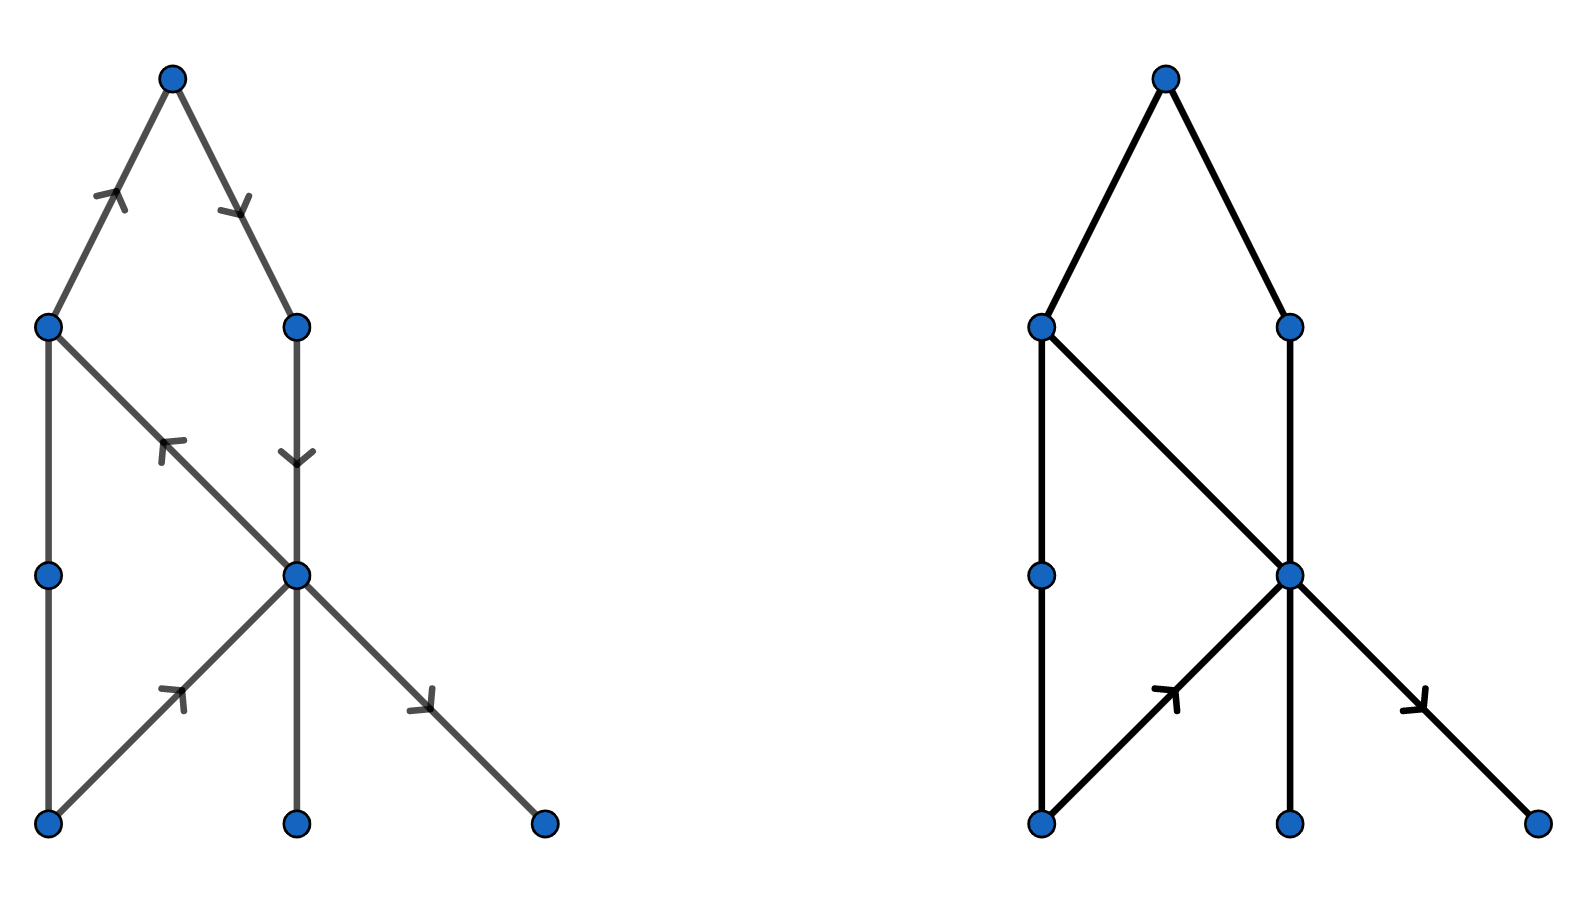
\includegraphics[width=0.6\linewidth]{poti.png}
        \caption{Primer poti ki sta blizu}
        \end{figure}

\begin{izrek}
    Naj bo $(X,x_0)$ končen pointed $T_0$ prostor. Potem je množenje $[\xi][\xi']=[\xi\xi']$ dobro definirano in inducira grupno strukturo na $\mathscr{H}(X,x_0)$
\end{izrek}

\begin{dokaz}
    Dobra definiranost in asociativnost sta očitni, enota je $[\emptyset]$. Naj bosta $\xi$ in $\xi'$ poti, $e$ $\h-$rob in $\mathfrak{e}(\xi)=\mathfrak{o}(\xi')=\mathfrak{o}(e)$. potem sta poti $[\xi \xi']$ in $[\xi e e^{-1} \xi']$, saj je $e$ monotona pot. Iz tega takoj sledi, da Da je inverz od $[e_1 e_2...e_n]$ enak $[e_n^{-1}...e_2^{-1}e_1^{-1}]$.
\end{dokaz}


\begin{izrek}
    Naj bo $(X,x_0)$ končen pointed $T_0$ prostor. Potem je grupa sklenjenih lomljenk $E(\k(X),x_0)$ izomorfna $\mathscr{H}(X,x_0)$.
\end{izrek}

\begin{dokaz}
    Definirajmo 
    \begin{align*}
\varphi:\mathcal{H}(X,x_0)&\rightarrow E(\k(X),x_0)\\
\langle e_1e_2...e_n\rangle&\mapsto [e_1e_2...e_n]\\
\emptyset &\mapsto [(x_0,x_0)]
    \end{align*}.

    Najprej pokažimo, da je $\varphi$ dobro definiran, torej da iz  $\langle e_1e_2...e_n\rangle =\langle f_1f_2...f_n\rangle $ sledi $[e_1e_2...e_n]=[f_1f_2...f_n]$.
    Naj bosta zanki $\xi_1 \xi_2 \xi_3 \xi_4$ in $\xi_1 \xi_4 $ blizu in naj bosta $\xi_2 = e_1e_2...e_n$ in $\xi_3 = e'_1e'_2...e'_m$ monotoni $\h-$poti. Potem velja 
\begin{align*}
    [\xi_1 \xi_2 \xi_3 \xi_4]&=[\xi_1 e_1e_2...e_{n-1}\mathfrak{o}(e_n)\mathfrak{e}(e_n) \xi_3 \xi_4]\\
    &=[\xi_1 e_1e_2...e_{n-2}\mathfrak{o}(e_{n-1})\mathfrak{e}(e_n) \xi_3 \xi_4]=\cdots=[\xi_1\mathfrak{e}(\xi_1)\mathfrak{e}(e_n) \xi_3 \xi_4]
\end{align*}
in analogno 
$$
[\xi_1\mathfrak{e}(\xi_1)\mathfrak{e}(e_n) \xi_3 \xi_4]=[\xi_1\mathfrak{e}(\xi_1)\mathfrak{e}(e_n) \mathfrak{o}(e'_1)\mathfrak{o}(\xi_4) \xi_4]
$$
in zato 
\begin{align*}
    [\xi_1 \xi_2 \xi_3 \xi_4]&=[\xi_1\mathfrak{e}(\xi_1)\mathfrak{e}(e_n) \mathfrak{o}(e'_n)\mathfrak{o}(\xi_4) \xi_4]\\
    &=[\xi_1(\mathfrak{e}(\xi_1)\mathfrak{e}(e_n)) (\mathfrak{e}(e_n)\mathfrak{e}(\xi_1)) \xi_4]=[\xi_1(\mathfrak{e}(\xi_1) \mathfrak{e}(\xi_1)) \xi_4]=[\xi_1 \xi_4].
\end{align*}


Obratno, če je $\xi =(x_0,x_1)(x_1,x_2)...(x_{n-1},x_n)$ lomljenka v $\k(X)$ z $x_0=x_n$, potem sta $x_i$ in $x_{i-1}$ primerljiva za vsak $1\leq i \leq n$, zato lahko najdemo monotone $\h-$poti $\xi_1, \xi_2,... \xi_n$, take da $\mathfrak{o}(\xi_{i-1})=\mathfrak{e}(\xi_i)$ za $1\leq i \leq n$. Definirajmo

\begin{align*}
    \psi: E(\k(X),x_0)&\rightarrow \mathcal{H}(X,x_0),\\
    [\xi]&\mapsto \langle\xi_1, \xi_2,... \xi_n\rangle.
\end{align*}

Definicija je neodvisna od izbire $\h-$poti $\xi_i$, saj če se izbiri razlikujeta za kak $i=k$, potem sta $\xi_1...\xi_k...\xi_n$ in $\xi_1...\xi'_k...\xi_n$ $\h-$ekvivalentni, saj sta obe blizu $\xi_1...\xi_k\xi_k^{-1}\xi_k...\xi_n$, torej $\langle \xi_1...\xi_k...\xi_n \rangle = \langle \xi_1...\xi'_k...\xi_n \rangle$

Definicija je neodvisna od izbire predstavnika. Recimo da sta $\xi(x,y)(y,x)\xi'$ in $\xi(x,z)\xi'$ ekvivalentni lomljenki v $\k(X)$, ki se začneta in končata v $x_0$, pri čemer sta $\xi$ in $\xi'$ lomljenki, $x,y$ in $z$ pa so primerljivi.
Če $y$ leži med $x$ in $z$, lahko najdemo monotono $\mathcal{H}-$pot od $x$ do $z$, ki vsebuje $y$ in nadomesti \pot od $x$ do $y$ in od $y$ do $z$ in zato je $\psi$ ekvivalentno definirana na $\xi(x,y)(y,x)\xi'$ in $\xi(x,z)\xi'$.
Če je $z\leq x \leq y$ lahko poiščemo monotone $\mathcal{H}-$poti $\alpha$ od $x$ do $y$ in $\beta$ od $z$ do $x$, potem bo $\overline{\alpha}\overline{\beta}$ nadomestila pot $(y,z)$ in $\overline{\beta}$ bo nadomestila pot $(x,z)$. Dokazati moramo le še, da velja $\langle\gamma \alpha \overline{\alpha}\overline{\beta}\gamma'\rangle=\langle \gamma\overline{\beta}\gamma\rangle$, za $\h-$poti $\gamma$ in $\gamma'$, kar je pa trivialno. Preostale kombinacije $x,y$ in $z$ dokažemo analogno.

Očitno sta $\varphi$ in $\psi$ drug drugemu inverzna in zato sta izomorfizma.
\end{dokaz}

Ker sta grupi $E(\k(X),x_0)$ in $\pi_1(|\k(X)|,x_0)$ izomorfni, takoj sledi naslednji rezultat.

\begin{posledica}
    Naj bo $(X,x_0)$ končen pointed $T_0$ prostor, potem $\pi_1(X,x_0)=\mathscr{H}(X,x_0)$.
\end{posledica}

\end{document}